\section{Dependency Grammar}
{\tiny curved arrows from the head to the dependent}\\
\scriptsize{auxiliary verbs}\\
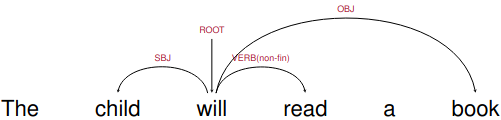
\includegraphics[scale=0.25]{auxiliary.png}\\
\scriptsize{Copular Clauses}\\
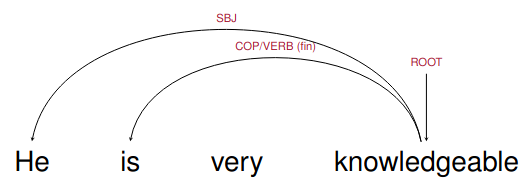
\includegraphics[scale=0.25]{copular.png}\\
\scriptsize{Dative Alternation}\\
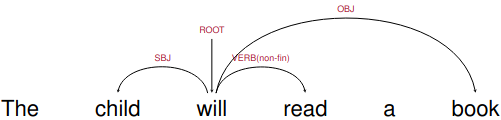
\includegraphics[scale=0.25]{auxiliary.png}\\
\scriptsize{Determiners} {\tiny DET, depends on the noun.}\\
\scriptsize{ADV} {\tiny depends on the verb or the ADV}\\
\scriptsize{ADJ} {\tiny depends on the noun}\\
\scriptsize{PP} {\tiny in PP, noun depends on preposition, other elements depend on the noun}\\
\scriptsize{POSS} {\tiny possessor depends on possessee}\\
\scriptsize{Complementizer Phrase} {\tiny complementizer (e.g. that) depends on the head-verb, itself is the head of the subordinate clause}\\
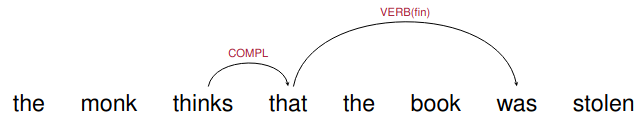
\includegraphics[scale=0.2]{complementizer.png}\\
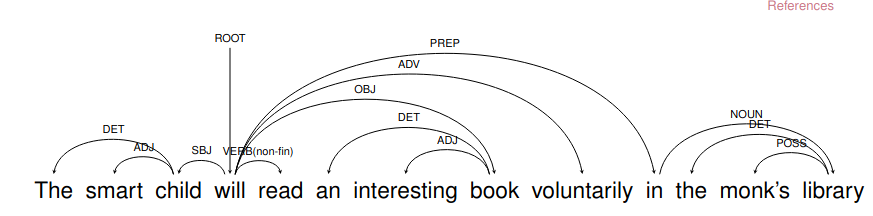
\includegraphics[scale=0.17]{DependencyGrammarExample.png}\\
\scriptsize{head-initial languages} {\tiny transitive sentences generally start with a verb, dependencies project forwards}\\
\scriptsize{head-final languages}
{\tiny dependencies project backwards}\\
\scriptsize{head-medial languages}
{\tiny dependencies project in both directions}\\
\scriptsize{linearization}
{\tiny dependency grammars often not not require particular rules
for the linearization of words; appropriate for languages with discontinuous constituents}\\
\scriptsize{free word order}
{\tiny linearization might not be required}\\
\scriptsize{fixed word order}
{\tiny lack of linearization constraints lincenses ungrammatical sentences}\\
\scriptsize{passive}\\
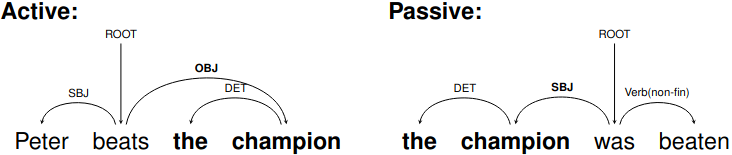
\includegraphics[scale=0.17]{passive.png}\\
\scriptsize{coordination}\\
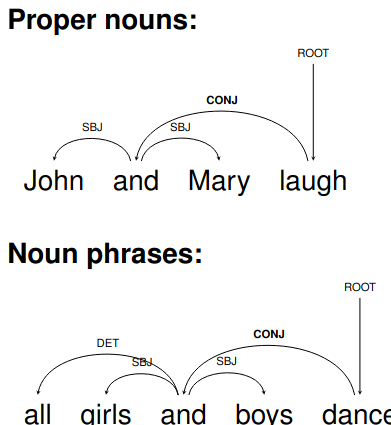
\includegraphics[scale=0.17]{coordination.png}\\
\scriptsize{crossing dependencies}
{\tiny non-projective}\\
\scriptsize{two competing pressures shpe word order}
{\tiny dependency length minimization; predictability maximization}